\documentclass[final,hyperref={pdfpagelabels=false}]{beamer}
\usepackage{grffile}
\mode<presentation>{\usetheme{I6pd2}}
\usepackage[english]{babel}
\usepackage[latin1]{inputenc}
\usepackage{amsmath,amsthm, amssymb, latexsym}
%\usepackage{times}\usefonttheme{professionalfonts}  % obsolete
%\usefonttheme[onlymath]{serif}
\boldmath
%\usepackage[orientation=portrait,size=a0,scale=1.4,debug]{beamerposter}
\usepackage[size=custom,width=121,height=91,scale=2,debug]{beamerposter}
% change list indention level
% \setdefaultleftmargin{3em}{}{}{}{}{}


%\usepackage{snapshot} % will write a .dep file with all dependencies, allows for easy bundling

\usepackage{array,booktabs,tabularx}
\newcolumntype{Z}{>{\centering\arraybackslash}X} % centered tabularx columns
\newcommand{\pphantom}{\textcolor{ta3aluminium}} % phantom introduces a vertical space in p formatted table columns??!!
\listfiles

\newcommand{\inv}{^{-1}}
\newcommand{\e}{\varepsilon}
\newcommand{\E}{\mathbb{E}}
\newcommand{\N}{\mathbb{N}}
\renewcommand{\P}{\mathbb{P}}
\newcommand{\R}{\mathbb{R}}
\newcommand{\X}{\mathcal{X}}
\newcommand{\Y}{\mathcal{Y}}
\newcommand{\Z}{\mathcal{Z}}
\newcommand{\dist}{\operatorname{dist}}
\newcommand{\vi}{{\vec i}}

%%%%%%%%%%%%%%%%%%%%%%%%%%%%%%%%%%%%%%%%%%%%%%%%%%%%%%%%%%%%%%%%%%%%%%%%%%%%%%%%%%%%%%
\graphicspath{{figures/}}
 
\title{\Large Exponential Concentration Inequality for a R\'enyi-$\alpha$
                                                        Divergence Estimator}
\author{Shashank Singh and Barnab\'as P\'oczos}
\institute[Carnegie-Mellon University]{Machine Learning Department,
                            Carnegie-Mellon University, Pittsburgh, PA, USA}
\date[June 22, 2014]{June 22, 2014}

%%%%%%%%%%%%%%%%%%%%%%%%%%%%%%%%%%%%%%%%%%%%%%%%%%%%%%%%%%%%%%%%%%%%%%%%%%%%%%%%%%%%%%
\newlength{\columnheight}
\setlength{\columnheight}{75cm}


%%%%%%%%%%%%%%%%%%%%%%%%%%%%%%%%%%%%%%%%%%%%%%%%%%%%%%%%%%%%%%%%%%%%%%%%%%%%%%%%%%%%%%
\begin{document}
\begin{frame}
  \begin{columns}
    % ---------------------------------------------------------%
    % Set up a column 
    \begin{column}{.32\textwidth}
      \begin{beamercolorbox}[center,wd=\textwidth]{postercolumn}
        \begin{minipage}[T]{.95\textwidth}  % tweaks the width, makes a new \textwidth
          \parbox[t][\columnheight]{\textwidth}{ % must be some better way to set the the height, width and textwidth simultaneously
            % Since all columns are the same length, it is all nice and tidy.  You have to get the height empirically
            % ---------------------------------------------------------%
            % fill each column with content            
            \vfill
            \begin{block}{Introduction}
              \begin{itemize}
              \item For a fixed $\alpha \in [0,1) \cup (1,\infty)$, we are
                    interested in estimating the R\'enyi-$\alpha$ divergence
                    \[D_\alpha(p\|q)
                        = \frac{1}{1 - \alpha} \log \int_\X
                                        p^\alpha(x)q^{1 - \alpha}(x)) \, dx,\]
                    between two unknown, continuous, nonparametric probability
                    densities $p$ and $q$ over $\X \subseteq \R^d$, using
                    samples from each density.
              \item Applications of divergence estimation include
                \begin{itemize}
                \item extending machine learning algorithms designed to operate
                      on finite-dimensional feature vectors to the setting
                      where inputs are sets or distributions.
                \item estimating entropy and mutual information.
                \end{itemize}
              \item R\'enyi-$\alpha$ Divergence has KL-Divergence as its
                    $\alpha \to 1$ limit case, and is related to
                    Tsallis-$\alpha$, Jensen-Shannon, and Hellinger
                    divergences.
              \item Few divergence estimators have known rates, and, to the
                    best of our knowledge, none have known exponential
                    concentration bounds.
%              \item Several important quantities enjoy this form:
%                \begin{itemize}
%                \item R\'enyi-$\alpha$ and Tsallis-$\alpha$ entropy, mutual
%                      information, and divergence
%                \item $f$-divergences
%                \item $L_p$ norms and divergence
%                \item Conditional versions of the above quantities
%                \end{itemize}
              \item We propose and analyze a plug-in estimator based on kernel
                    density estimation, for densities on the unit cube
                    $\X = [0,1]^d$. We prove
                \begin{itemize}
                \item the estimator is exponentially concentrated about its
                      mean.
                \item for densities in a $\beta$-H\"older smoothness class with
                      certain boundary conditions, the bias of the estimator is
                      bounded by
                      $O\left( n^{-\frac{\beta}{\beta + d}} \right)$, where $n$
                      is the number of samples from each density.
                \end{itemize}
              \end{itemize}
            \end{block}
%            \vfill
%            \begin{block}{Problem Statement}
%            {\footnotesize
%            Given a positive integer $d$, consider two probability densities
%            $p,q : \X = [0,1]^d \to \R$ on the unit cube, with known positive
%            lower and upper bounds $\kappa_1,\kappa_2 \in \R$
%            ($0 < \kappa_1 \leq p,q \leq \kappa_2 < \infty$). For a given
%            $\alpha \in [0,1) \cup (1,\infty)$, we are interested in using
%            random samples of $x^1,\dots,x^n \in \X$ and $y^1,\dots,y^n$ of $n$
%            i.i.d. points from $p$ and $q$, respectively, to estimate
%            $D_\alpha(p\|q)$.}
%\begin{enumerate}[]
%\item
%\end{enumerate}
%\vspace{-10mm}
%            \end{block}
            \vfill
            \begin{block}{Assumptions}
              {\footnotesize
              Let $\beta > 0$, and let $\ell := \lfloor \beta \rfloor$ be
              the greatest integer \emph{strictly} less than $\beta$. We make
              the following four assumptions on the densities $p$ and $q$, and
              the kernel $K$:\\}
              \begin{itemize}
              \item {\bf\footnotesize (Smoothness)} All (mixed)
              $\ell$-order partial derivatives of $p$ and $q$ exist and are
              $(\beta - \ell)$-H\"older Continuous (i.e., $\exists L \in \R$
              such hat, $\forall x, x + v \in \X$, $|\vi| = \ell$,
                    \[|D^\vi p(x + v) - D^\vi p(x)|,
                      |D^\vi q(x + v) - D^\vi q(x)|
                                        \leq L\|v\|_2^{\beta - \ell}\mbox{)}.\]
              \item {\bf\footnotesize (Boundedness)}
                    $\exists \kappa_1,\kappa_2 \in \R$ such that,
                    $\forall x \in \X$,
                    \[0 < \kappa_1 \leq p(x),q(x) \leq \kappa_2 < +\infty.\]
              \item {\bf\footnotesize (Boundary)} All derivatives of
                    $p$ and $q$ vanish at the boundary
                    \[\partial\X = \{x \in \X : x_i \in \{0,1\}
                                            \mbox{ for some } i \in [d]\}\]
                    (i.e., $\sup_{1 \leq |\vi| \leq \ell} |D^\vi(x)| \to 0$
                    as $\dist(x,\partial\X) \to 0$).
                    \vspace{1cm}
              \item {\bf\footnotesize (Kernel)} The kernel
                    $K : \R \to \R$ has support in $[-1,1]$,
                    \[\hspace{-15mm}\int_{-1}^1 K(u) \, du = 1
                                    \quad \mbox{ and } \quad
                                    \int_{-1}^1 u^j K(u) \, du = 0,
                                    \quad
                                    \forall j \in \{1,\dots,\ell\}.\]
              \end{itemize}
            \end{block}
            \vfill
          }
        \end{minipage}
      \end{beamercolorbox}
    \end{column}
    % ---------------------------------------------------------%
    % end the column

    % ---------------------------------------------------------%
    % Set up a column 
    \begin{column}{.32\textwidth}
      \begin{beamercolorbox}[center,wd=\textwidth]{postercolumn}
        \begin{minipage}[T]{.95\textwidth} % tweaks the width, makes a new \textwidth
          \parbox[t][\columnheight]{\textwidth}{ % must be some better way to set the the height, width and textwidth simultaneously
            % Since all columns are the same length, it is all nice and tidy.  You have to get the height empirically
            % ---------------------------------------------------------%
            % fill each column with content
            \vfill
            \begin{block}{Mirrored Kernel Density Estimator}
              \begin{columns}
                \begin{column}{.63\textwidth}
                  {\footnotesize
                  Given a bandwidth $h$, our R\'enyi-$\alpha$ divergence
                  estimate is computed in 3 steps:}
                  \begin{enumerate}
                  \item Mirror data over subsets of edges of $\X$.
                  \item Compute clipped kernel density estimates $\hat p$ and
                        $\hat q$ from the mirrored data, using product kernel
                        $K_d$ and bandwidth $h$, and clipping the kernel
                        density estimates pointwise below at $\kappa_1$ and
                        above at $\kappa_2$.
                  \item Estimate $D_\alpha(p\|q)$ by the plug-in estimator
                        $D_\alpha(\hat p\|\hat q)$.
                  \end{enumerate}
                \end{column}
                \begin{column}{.36\textwidth}
                  \begin{figure}[h!]
                    \centering
                    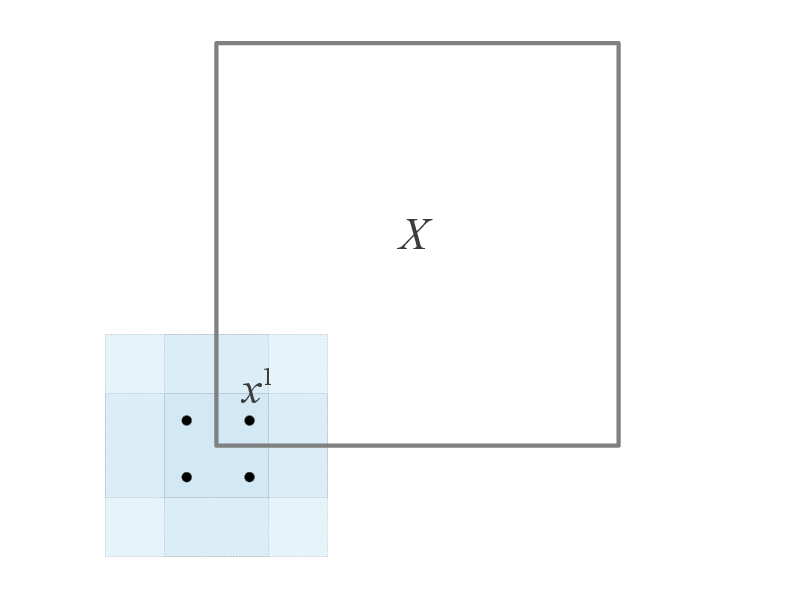
\includegraphics[width=\linewidth]{figures/mirror_fig}
                    \caption{\scriptsize Four kernels centered on a single data
                                         point and its three reflected copies,
                                         in the case $d = 2$.}
                    \label{fig:mirror_fig}
                  \end{figure}
                \end{column}
              \end{columns}
            \end{block}
            \vfill
            \begin{block}{\normalsize Results: Exponential Concentration Bound}
              \begin{itemize}
              \item We show that, $\forall \e > 0$,
                \[\P\left(
                        \left| D_\alpha(\hat p \| \hat q)
                           - \E D_\alpha(\hat p \| \hat q) \right|
                        > \e
                    \right)
                    \leq 2\exp\left( -C_V^2\e^2n \right),\]
              where
              \vspace{-5mm}
\[C_V = \frac{|\alpha - 1|}{2C_fC_L\|K\|_1^d}\]
              is constant in $n$ and $h$.
              \item Main tool in proof is McDiarmid's Inequality, by which it
              suffices to bound the change in the estimate when resampling a
              single data point by $C_V/n$.
              \item This is achieved by combining a smoothness property of
              $D_\alpha$ with the observation that the integral of the
              mirrored kernel density estimate changes by at most
              $\frac{2}{n} \int_{[-1,1]^d} |K^d(u)| \, du$.
              \end{itemize}
            \end{block}
            \vfill
            \begin{block}{Bias Lemma}
              \begin{itemize}
              \item {\bf\footnotesize Bias Lemma:} Writing the pointwise bias
                    of the clipped and mirrored kernel density as
                    $b_p(x) = \E \hat p(x) - p(x)$, we show
                    \[\int_\X b_p^2(x) \, dx \leq C_b h^{2\beta}.\]
                    \begin{itemize}
                    \item For somewhat small $h$ and large $\beta$ (in
                    particular, $h \leq \sqrt\frac{1}{3d^{1/r}}$ and
                    $\beta \geq 6d + 2$ suffices), one can show $C_b \leq 3L$.
              \item Away from the boundary of $\X$ (i.e., in $[h,1 - h]^d$),
                    there is no boundary bias, and so we simply cite well-known
                    results in kernel density estimation, using the assumed
                    symmetry properties of the kernel.
              \item For $x$ near (within $h$ of) the boundary of $\X$, we
                    combine the Smoothness and Boundary Conditions via a Taylor
                    bound to derive a pointwise bound $b_p(x) \leq C_bh$.
                    \end{itemize}
              \end{itemize}
            \end{block}
            \vfill
          }
        \end{minipage}
      \end{beamercolorbox}
    \end{column}
    % ---------------------------------------------------------%
    % end the column

    % ---------------------------------------------------------%
    % Set up a column 
    \begin{column}{.32\textwidth}
      \begin{beamercolorbox}[center,wd=\textwidth]{postercolumn}
        \begin{minipage}[T]{.95\textwidth} % tweaks the width, makes a new \textwidth
          \parbox[t][\columnheight]{\textwidth}{ % must be some better way to set the the height, width and textwidth simultaneously
            % Since all columns are the same length, it is all nice and tidy.  You have to get the height empirically
            % ---------------------------------------------------------%
            % fill each column with content
            \vfill
            \begin{block}{Results: Convergence Rate}
              \begin{itemize}
              \item We show there exists $C_B \in \R$ (constant in $n$ and $h$)
                    such that
                    \[|\E D_\alpha(\hat p\|\hat q) - D_\alpha(p\|q)|
                    \leq C_B\left( h^\beta + \frac{1}{nh^d} \right).\]
              \item Proven by making a second-order Taylor estimate and then
                    using H\"older's Inequality to reduce terms to the Bias
                    Lemma and the integrated mean squared error of a standard
                    kernel density estimator.
              \end{itemize}
            \end{block}
            \vfill
            \begin{block}{Discussion}
                  \begin{itemize}
                  \item The exponential concentration bound gives a bound on
                        the variance of the estimator:
                        \vspace{-5mm}
                        \[\mathbb{V}[F(\hat p_1,\dots,\hat p_k)]
                                                    \leq C_V^2n\inv.\]
                  \item This does not depend on $h$, so pick $h$ to minimize
                        the bias bound.
                        \begin{itemize}
                        \item Asymptotically optimal $h$ is
                              $h \asymp n^{-\frac{1}{\beta + d}}$, so bias
                              bound is
                              $O\left( n^{-\frac{\beta}{\beta + d}} \right)$.
                        \end{itemize}
                  \item Hence MSE is $O(n^{-\frac{\beta}{\beta + d}} + n\inv)$,
                        which is the parametric rate $O(n\inv)$ if
                        $\beta \geq d$ and $O(n^{-\frac{\beta}{\beta + d}})$
                        otherwise.
                  \item Kernel assumptions for the bias bound necessitate
                        $\|K\|_1 > 1$ when $\beta \geq 2$ and $C_V$ includes
                        $\|K\|_1^d$, which is exponential in $d$.
                        \begin{itemize}
                        \item Lower bounds in $d$ are unknown; whether
                        dependence is necessarily exponential is an important
                        open problem.
                        \end{itemize}
                  \end{itemize}
            \end{block}
%            \vfill
%            \begin{block}{The R\'enyi-$\alpha$ Divergence and Conditional
%                                                    Mutual Information Cases}
%            Fix $\alpha \in [0,1) \cup (1,\infty)$. Two particular density
%            functionals of interest are R\'enyi-$\alpha$ Divergence
%            \[D_\alpha(p_1\|p_2) = \frac{1}{1 - \alpha} \log
%                        \int_{\X} p_1^\alpha(x)p_2^{1 - \alpha}(x) \, dx,\]
%            where $p_1$ and $p_2$ are densities, and R\'enyi-$\alpha$
%            Conditional Mutual Information
%            \begin{align*}
%            & I_\alpha(X;Y | Z) \\
%            & = \int_\Z \frac{P(z)}{1 - \alpha} \log
%            \int_{\X \times \Y} \left( \frac{P(x,y,z)}{P(z)} \right)^\alpha
%            \left( \frac{P(x,z)P(y,z)}{P^2(z)} \right)^{1 - \alpha}
%            \hspace{-20mm} d(x,y) dz,
%            \end{align*}
%            where $X$, $Y$, and $Z$ are random variables and $P$ denotes their
%            joint density, as well as its marginal densities.
%            \end{block}
            \vfill
            \begin{block}{Experimental Results on Synthetic Data}
              \begin{columns}
                \begin{column}{.5\textwidth}
                  \begin{itemize}
                  \item $\displaystyle
                          \vec\mu_1 = \begin{bmatrix} 0.3\\0.3\\0.3 \end{bmatrix},
                          \vec\mu_2 = \begin{bmatrix} 0.7\\0.7\\0.7 \end{bmatrix}$
                  \item $\displaystyle
                          \Sigma = \begin{bmatrix}
                                      0.2 & 0   & 0   \\
                                      0   & 0.2 & 0   \\
                                      0   & 0   & 0.3
                                   \end{bmatrix}$
                  \item $p_1 = \mathcal{N}(\vec\mu_1,\Sigma),
                         p_2 = \mathcal{N}(\vec\mu_2,\Sigma)$
                  \item In each trial, $n$ points were drawn from $p_1$ and
                        $p_2$ restricted to $[0,1]^3$.
                        $D_\alpha(\hat p \| \hat q)$ was computed from the
                        samples and $D_\alpha(p_1\|p_2)$ was computed directly.
                  \end{itemize}
                \end{column}
                \begin{column}{.49\textwidth}
                  {\footnotesize
                  Mean squared error and standard deviation of our
                  estimator were computed from 100 trials and plotted below.}
                  \begin{enumerate}[]
                  \item
                  \end{enumerate}
                 \vspace{-10mm}
                  \begin{figure}[h!]
                    \centering
                    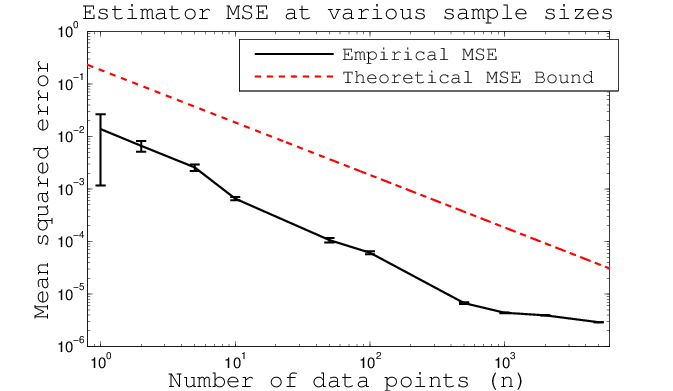
\includegraphics[width=\linewidth]{figures/MSE}
                    \caption{\scriptsize{Log-log plot of mean squared (computed over 100
                            trials) for various sample sizes $n$, alongside our
                            theoretical bound. Error bars indicate standard
                            deviation of estimator over 100 trials.}}
                    \label{fig:exp_res}
                  \end{figure}
                \end{column}
              \end{columns}
            \end{block}
          }
          % ---------------------------------------------------------%
          % end the column
        \end{minipage}
      \end{beamercolorbox}
    \end{column}
    % ---------------------------------------------------------%
    % end the column
  \end{columns}
  \vskip1ex
  %\tiny\hfill\textcolor{ta2gray}{Created with \LaTeX \texttt{beamerposter}  \url{http://www-i6.informatik.rwth-aachen.de/~dreuw/latexbeamerposter.php}}
  {\tiny\hfill\LaTeX \texttt{beamerposter}  \url{http://www-i6.informatik.rwth-aachen.de/~dreuw/latexbeamerposter.php} \hskip1em}
\end{frame}
\end{document}


%%%%%%%%%%%%%%%%%%%%%%%%%%%%%%%%%%%%%%%%%%%%%%%%%%%%%%%%%%%%%%%%%%%%%%%%%%%%%%%%%%%%%%%%%%%%%%%%%%%%
%%% Local Variables: 
%%% mode: latex
%%% TeX-PDF-mode: t
%%% End:
